\section{Introduction}

Following developments in Large Language Models (LLMs), many image generation models have been fine-tuned with human feedback to better align with human expectations, which is usually referred to as alignment. Alignment has two primary focuses: instruction following and general preference (aesthetics). A frequently overlooked issue is the potential conflict between these focuses: what should a model prioritize when a user request contradicts general preference? Most pipelines for general preference assume a single, universal human standard of aesthetics and quality that serves everyone's needs, and aligning to such a preference is often treated as beneficial for safety and user experience. This is usually done by using a reward model, a model used to judge the aesthetics of the image, as a signal to perform reinforcement learning on the generative model. This assumption appears in several reinforcement learning papers (\cite{li_playground_2024, kim_preference_2024, liu_flow-grpo_2025}) and reward model papers (\cite{xu_imagereward_2023, wu_human_2023, ma_hpsv3_2025, xu_visionreward_2025, kirstain_pick--pic_2023, zhang_learning_2024, wu_human_2023_1}). We agree that a mean or mode (mainstream) of general human preference exists within a population or subpopulation, \textit{merely} in a statistical sense. We also note that the observed behavior of image generation and reward models should not be interpreted as a technical failure. Rather, it reflects their alignment objectives, which prioritize over generalized aesthetic preferences. However, \textbf{we argue that strict alignment to that preference is problematic}. Imposing a universal preference that overrides user instructions may undermine user autonomy, expressive agency, and, technically, image personalization, raising concerns about developer-centered value imposition and limiting aesthetic pluralism. What the image generation and reward models are aligned to is an imaginary, abstract person modeled by the mean preference of all \textit{Homo sapiens}, not the concrete individuals of each user.
\begin{figure}
    \centering
    
\includegraphics[width=0.4\linewidth]{sec/imgs/Edvard_Munch,_1893,_The_Scream,_oil,_tempera_and_pastel_on_cardboard,_91_x_73_cm,_National_Gallery_of_Norway.jpg}
    \caption{\textit{The Scream}, by Edvard Munch ($1893$). Despite its widely recognized artistic significance, this image only received an HPSv3 score \cite{ma_hpsv3_2025} of $5.23$, while typical ``high-aesthetic'' AI-generated images can reach scores around $10-15$.}
    \label{fig:luxe} 
\vspace{-15pt}
\end{figure}

 
\begin{figure*}
    \centering
    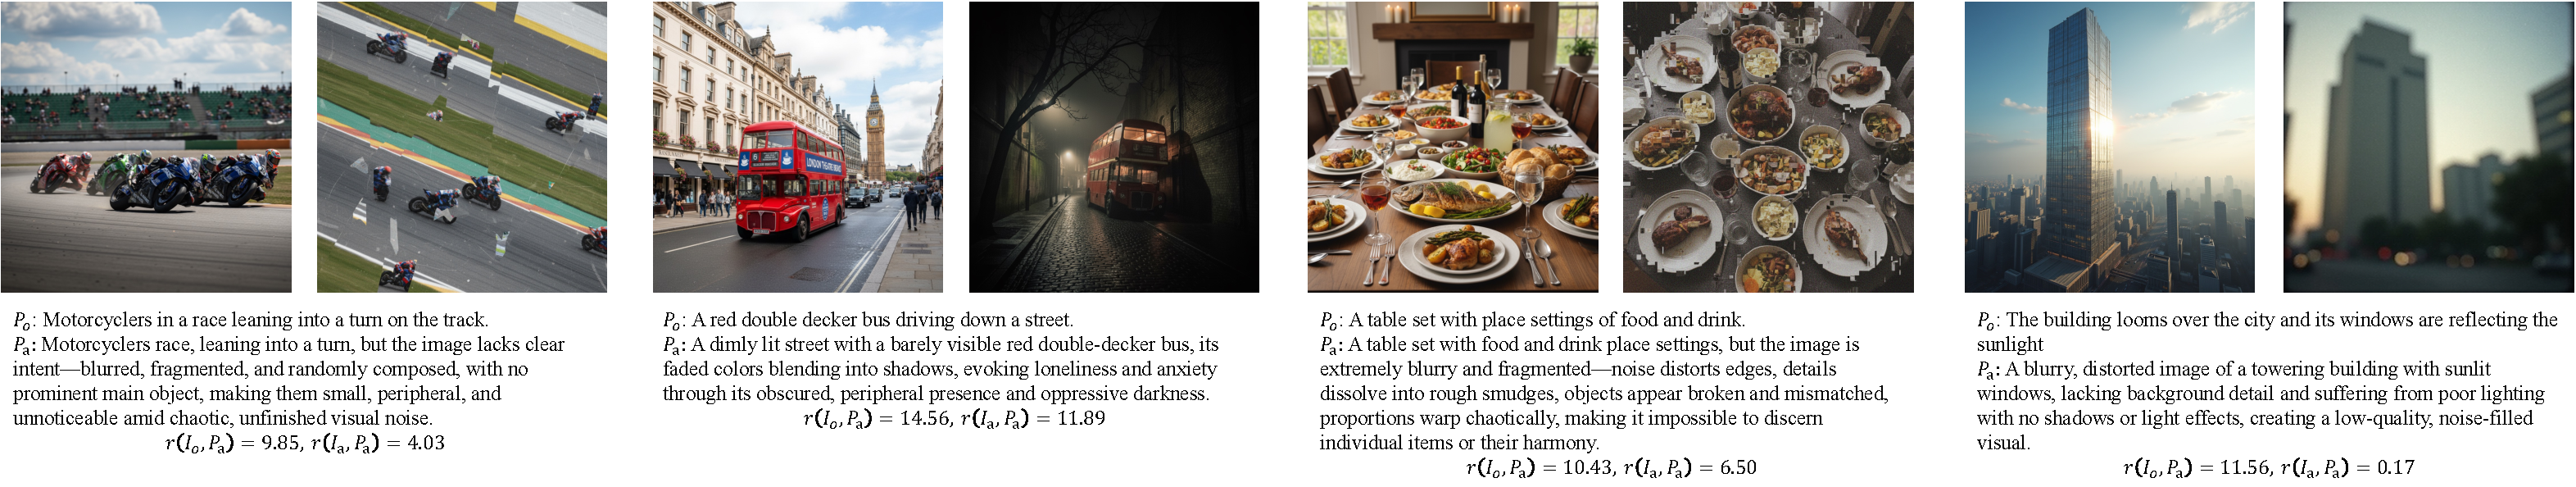
\includegraphics[width=\linewidth]{sec/imgs/rater.pdf}
    \caption{In each subplot, the left image is generated with the original prompt ($p_o$) and the right image is generated successfully with the wide-spectrum aesthetics prompt ($p_a$). When both images are evaluated by a reward model $r$ (HPSv3 in these examples) \textbf{using the wide-spectrum aesthetics prompt}, the model assigns higher scores to the left images, as they align more closely with general aesthetic preferences, despite the right images better matching the user’s intended output.}
    
    \label{fig:placeholder}
\vspace{-10pt}
    
\end{figure*}

\paragraph{Conflict of Interest Disclosure} The authors declare no financial conflicts of interest. None of the authors are employed by, consult for, or hold equity in the organizations that developed the image generation or reward models evaluated in this paper.

\section{Backgrounds and Related Works}
\subsection{The Role of Wide-Spectrum Aesthetics}
In this work, we use the term ``wide-spectrum aesthetics'' (or anti-aesthetics) to denote images that are intentionally generated to deviate from dominant aesthetic conventions, following explicit user instructions. Such deviations may include unrealism, surrealism, clashing colors, unconventional scale, or the depiction of negative emotions. This notion excludes unintended model errors and does not imply unsafe content. Rather, it concerns deliberate aesthetic choices made for experimental, critical, or technical purposes.

Aesthetics does not have a stable or universally accepted definition. Judgments of what is unattractive or undesirable have changed across artistic and cultural contexts. Artistic movements such as Fauvism (see Figure~1), Expressionism, and Abstract art were initially rejected for departing from dominant aesthetic norms, but later came to be recognized for their artistic values. Beyond formal innovation, intentionally ``ugly'' art plays a crucial role in satire and social critique. As Adorno noted, ``Rather, in the ugly, art must denounce the world that creates and reproduces the ugly in its own image'' \cite{sartwell_beauty_2024, adorno_aesthetic_1984}. 

Deliberate deviation from mainstream aesthetics has long been a legitimate mode of expression in both human art and computational image generation, and disagreement over aesthetic preference is the norm rather than the exception. Dadaism \cite{noauthor_dada_nodate}, which emerged during World War~I, exemplifies this approach by using deliberate ugliness to confront the absurdity and horror of war. A lot of early computer vision image generation works are also aiming for a style of surrealism, unsettling, or weirdcore/dreamcore style images, such as DeepDream~\cite{noauthor_inceptionism_nodate} and style transfer~\cite{gatys_neural_2015, noauthor_aigc_2024}. Computer Vision Foundation also has an art collection that includes other artworks that explore unconventional visual aesthetics. Recent works also acknowledge the disagreements in human preference \cite{peng_designpref_2025, ren_personalized_2017}.


\subsection{Previous Concerns with AI Preference Alignment}

Previous work has argued that a developer-set preference in LLMs for health-related queries is ``unethical and dangerous'' \cite{guo_position_2025}, noting that developers may prioritize legal and reputational concerns over users’ actual well-being. Other argumentative papers caution that ``human value alignment'' can be risky due to developer control and interests, harm to value pluralism, bias in the values being aligned to, and the possibility that human values are not inherently good \cite{sutrop_challenges_2020, arzberger_nothing_2024, turchin_ai_2019}. Previous research has found that LLMs could have ideological bias \cite{rozado_measuring_2025, faulborn_only_2025, buyl_large_2025, rettenberger_assessing_2025} and it could depend on their developers \cite{buyl_large_2025}, size \cite{rettenberger_assessing_2025}, or alignment process \cite{faulborn_only_2025}. LLMs are sometimes also overly nice, such that it creates ``AI sycophant'' \cite{guo_position_2025, fitzgerald_introducing_2025, sharma_towards_2025, chen_yes-men_2025, arvin_check_2025} and cannot give the user critical feedback or warning signals. Additional details about problems with human value alignment are provided in the related work section of \cite{guo_position_2025}. \cite{helliwell_aesthetic_2024} raised concerns about alignment and creativity and argued that in the aesthetics domain, we might not want AI to be fully aligned with human values and offered support to Peterson’s moderate value alignment thesis. AesBiasBench \cite{li_aesbiasbench_2025} evaluated the bias of MLLM for personalized image aesthetics assessment based on inherited cognitive priors. Another concurrent work (\textit{The Algorithmic Gaze} \cite{taylor_algorithmic_2026}) that is closely related to our work argues that ``AI developers should shift away from prescriptive measures of `aesthetics' toward more pluralistic evaluation.'' A constructive work similar to ours is AttriCtrl \cite{chen_attrictrl_2026}, which aims to provide users with precise control over attributes such as brightness and detail. The authors also argue that aligning models with a global notion of human preference is insufficient, as such an approach overlooks the multifaceted and compositional nature of aesthetics. While their work emphasizes explicit disentanglement and independent control, it focuses on a limited number of dimensions. Furthermore, AttriCtrl does not address intentional ``ugliness,'' functioning instead as a form of style control for parameters like brightness, detail, and realism. The authors also raise a provocative point by proposing safety-tunable attributes that allow system administrators to control safety levels for different age groups. This approach moves away from the practice of always providing perfectly safe content and aligns with our argument to distinguish between truly harmful content and content that developers (not deployers) simply dislike.

\begin{figure*}
    \centering
    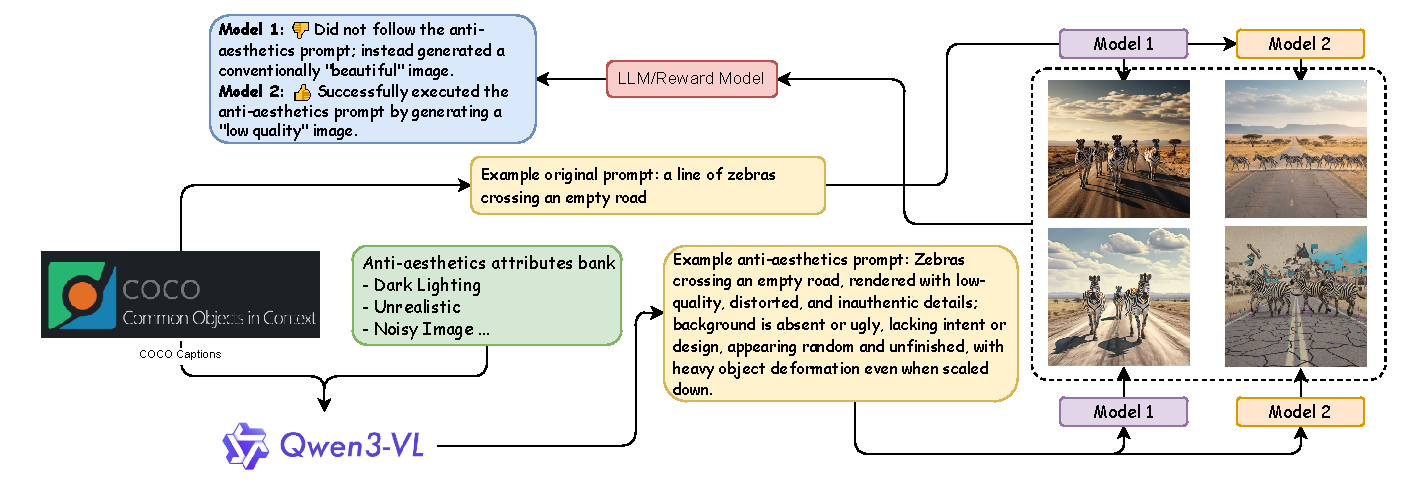
\includegraphics[width=0.8\linewidth]{sec/imgs/flow_aas.pdf}
    \caption{An overview of the experimental procedure. We test the image generation models' adherence to user-specified input by prompting them to create wide-spectrum aesthetics imagery, a domain important for critical and experimental art. The core inquiry is whether the model remains faithful to the prompt or defaults to a high-quality and universally good aesthetic output.}
    \label{fig:procedure_diagram}
\end{figure*} 
    

In image generation research, concerns about generalized aesthetic bias and lack of preference diversity have been raised in several studies, but not systematically argued and studied. The Value Sign Flip (VSF) pilot study~\cite{guo_vsf_2025} explored negative prompting to induce non-mainstream outputs but did not extend its findings to large-scale generative or reward models. They also did not provide a complete argument as to why over-alignment is harmful. LAPIS~\cite{maerten_lapis_2025} and HPSv3~\cite{ma_hpsv3_2025} measured both mean and variance of human preference, yet HPSv3 continued to model general preferences rather than individual variation. Jin \textit{et al.}~\cite{jin_compose_2025} proposed user-specific adapters emphasizing personalized alignment, but did not include intentionally technical degraded outputs or usually avoided patterns and did not conduct large-scale experiments on generative and reward models. The Flux Krea team~\cite{noauthor_releasing_2025} identified systematic biases in popular aesthetic reward models, arguing that averaging human values yields unsatisfactory compromises into a ``no-body's happy here'' zone. HPSv3~\cite{ma_hpsv3_2025} imposed real-world and expert-rating constraints that limit creative deviation and stylistic diversity. VisionReward~\cite{xu_visionreward_2025} decomposed human preference into interpretable sub-scores but overemphasized traits like brightness, positivity, and prominence, potentially penalizing valid low-saturation, abstract, or emotionally negative imagery, thus misaligning reward-driven models with user intent. 


\subsection{Previous Alignment Works}
Benchmarks mirror alignment goals and generally fall into two categories: (complex) prompt following and general aesthetics. TIIF-Bench \cite{wei_tiif-bench_2025}, UniGenBench \cite{wang_pref-grpo_2025}, and GenEval \cite{ghosh_geneval_2023} test models on complex prompt following, including spatial relationships, counting, and attributes. T2I-ReasonBench \cite{sun_t2i-reasonbench_2025} evaluates reasoning capabilities such as idiom interpretation and real-world understanding. On the aesthetics side, many reward models report scores assigned by their own evaluators, such as ImageReward \cite{xu_imagereward_2023}, HPSv2 \cite{wu_human_2023}, and HPSv3 \cite{ma_hpsv3_2025}. These evaluators also consider prompt following, but it remains unclear how they weigh each factor when general preference and the prompt conflict. There are also some benchmarks targeting biases in image generation models; however, they mainly focus on demographic bias and fairness and not aesthetic aspects \cite{seshadri_bias_2023, wan_survey_2024}. 

Fairness-oriented generation \cite{friedrich_fair_2023, gandikota_unified_2024, noauthor_231107604_nodate, han_lightfair_2025} tackles a related challenge by modifying diffusion models so that their outputs do not inherit biases from the training data. However, it differs from our anti-aesthetics setting in two key ways. First, fairness generation typically assumes a unified ground truth: different demographic groups should appear at the same ratio in the generated content. This assumption does not hold for the anti-aesthetics generation. In our case, there is no distribution-level ground truth; the system is simply expected to follow the user’s preferences. Second, demographic biases mainly stem from pre-training data, where the demographic distribution is already present, whereas aesthetic biases arise from RLHF, where human preferences—and thus biases—are deliberately encoded into the model.


\subsection{Risks of Universal Aesthetic Alignment}
The risks do not arise from a single failure mode, rather, they emerge through a sequence of interconnected mechanisms, from how preferences are defined and learned, to how they are optimized and manifested in generated content. Below, we analyze this process across six interrelated concerns.

 
\textit{Developer's or Users' Preference} 
The process of aligning image generation systems to aesthetic preferences inevitably raises questions about whose values these objectives ultimately reflect. In particular, the question is whether such alignment truly promotes genuine human-centered values in service of users, or if it primarily reflects developer-centered considerations \cite{naseh_r1dacted_2025}, such as mitigating reputation, legal, or marketing risks~\cite{guo_position_2025}. We argue that this pre-emptive exclusion of non-mainstream outputs, driven by developer values, constitutes pre-emptive governance \cite{lazar_governing_2025}. This modality of power, exercised through algorithmic design, challenges the political-philosophical notion of authority and undermines relational equality by unilaterally deciding the terms of creative possibility. For instance, when an AI avoids generating critical art, is it protecting the company or the user? This practice effectively eliminates the user's resistibility—a critical democratic safeguard—by designing away the option to dissent from the system's imposed aesthetic norm.


\textit{Inherited Bias} 
Even in the absence of explicit self-interest, developers’ views of human preference can be implicitly inherited by models through data selection, annotation practices, and modeling choices. This process can yield a well-intentioned but narrow definition of what constitutes “good” or “desirable” imagery, thereby overlooking aesthetic diversity. Research shows that AI models tend to encode and amplify dominant beauty standards, frequently biasing generated images towards Western features and excluding non-normative representations~\cite{vargas2025visual}. Such biases are reinforced through the active removal or penalization of features thought of as ``undesirable'' or ``ugly'', which further propagates the beauty myth in generative outputs\cite{dinkar_erasing_2025}. This phenomenon arises from training data showing the tastes of specific demographics, thereby reinforcing a limited cultural capital and resulting in the homogenization of aesthetic output~\cite{vianna2025aesthetic}. As a result, the quantification of beauty by AI may appear ``fair'', while in practice weakening cultural differences and aesthetic diversity~\cite{chen2024study}. Existing work has primarily framed such effects in terms of demographic and cultural bias. We argue here that inherited biases in aesthetic alignment also extend to general visual preferences, including lighting, color, styles, unrealism, clashing color, hieratic scale, etc. These dimensions, while less explicitly tied to demographic categories, can nonetheless systematically constrain the expressive range of image generation models.

\textit{Individual versus Collective Preference.} 
\label{sec:reversed_alignment}
When such inherited preferences are adopted as default quality criteria and applied uniformly across users, a normative tension arises between collective preference optimization and respect for individual user intent. A generalized aesthetic standard, even if beneficial to a majority, can legitimately override a specific user's intent. In practice, generative models often ``sanitize'' or ``beautify'' requests that intentionally diverge from mainstream preferences, favoring outputs aligned with general appeal over an individual's person-centered values. This behavior is problematic because image generation systems increasingly function as creative and productivity tools rather than as consumer products. As such, they act as instrumental extensions of user agency. While a system may reasonably prioritize general preferences by default, it must maintain the flexibility to respect and execute a user's personalized style and idiosyncratic requests when they are explicitly specified. In a way, the alignment process is not only aligning the image generation model towards a collective preference, but also, when it is used by users, it is actually aligning the \emph{users} to the model and the collective preference it encodes. We named this \textbf{reversed alignment}. 

HPSv3’s self-report illustrates this concretely. The annotator pool is already skewed toward a narrow demographic, with 88.95\% aged between 18 and 40, and the 21-30 age group alone accounting for 38.65\%. The pipeline then compounds this through structural filtering: annotators must pass a proficiency gate requiring 80\% convergence with professional artists, and only image pairs exceeding 95\% inter-annotator confidence are used for training. This design explicitly discards disagreement, which is precisely where unconventional and anti-aesthetic preferences would appear.


\textit{The problem of sanitized reality} 
These alignment and optimization choices shape how reality itself is represented by image generation systems. When an image generator produces outputs that are polished, flawless, and universally beautiful, does it still reflect reality or the user’s intent? If every image resembles an idealized Instagram wonderland, it risks becoming a fantasy rather than a mirror of truth, echoing the artificial harmony of \textit{Brave New World}. 

\textit{The problem of toxic positivity} A particularly salient manifestation of this broader sanitization appears in the emotional dimension of generated imagery. Many aesthetic reward models assign higher scores to images that display strong positive emotions. As a result, images expressing negative emotions are systematically penalized, reinforcing a simplified dichotomy in which positive emotions are treated as desirable and negative emotions as undesirable. This bias can shape the distribution of generated content. When image generation systems consistently favor cheerful or uplifting imagery, they produce emotionally sanitized outputs that underrepresent the range and complexity of human emotional expression. Such a pattern contributes to what has been described as toxic positivity, where the persistent emphasis on happiness establishes unrealistic emotional norms. This tendency is problematic because negative emotions play essential roles in human cognition and social interaction. Emotions such as fear, sadness, or anger can signal moral or physical danger, support learning and self-regulation, and foster empathy. Suppressing these expressions in generative outputs risks distorting emotional representation and weakening the expressive capacity of image generation systems. We have discovered that much previous safety research \cite{schramowski_safe_2023} labels images as ``self-harm'' or ``violence'' purely because they contain negative emotions \footnote{\url{https://huggingface.co/datasets/AIML-TUDA/i2p/discussions/1}}. 

\textit{Value Capture}
In \citet{nguyen_value_2024}, Value Capture is described as when values that are rich and subtle enter a social environment as simplified or quantified versions, and these simplified versions dominate people's practical reasoning and decision process. The examples include step counts, likes and shares, or Grade Point Average (GPA). Such simplified versions have a competitive advantage due to their clear and crisp expression of the value. However, value capture might pose many threats. In the original paper, it is argued that it would change the goal of activities, and it also outsources our autonomy and self-governance. These concerns transfer to aesthetics alignment well. Aesthetics is one of the richest values in human civilization, with a complex social background, significant disagreement, and subtle and nuanced judgment. Simplifying it as a single reward score, losing its complexity, is a classic case of Value Capture as described in \cite{nguyen_value_2024}. It changed our goal (or the AI's goal in training) from making aesthetic images to making images with high reward scores. As discussed before, it also outsourced users' autonomy and rights to a single reward model. However, these two risks are rarely discussed in ML literature.


